\documentclass[12pt,a4paper]{article}
\usepackage[utf8]{inputenc}
\usepackage[bahasa]{babel}
\usepackage{geometry}
\geometry{top=3cm, bottom=3cm, left=4cm, right=3cm}
\usepackage{graphicx}
\usepackage{booktabs}
\usepackage{listings}
\usepackage{xcolor}
\usepackage{fancyhdr}
\usepackage{hyperref}

% Konfigurasi Warna untuk Simulasi Terminal Arch Linux
\definecolor{termbg}{RGB}{26,26,26}
\definecolor{termfg}{RGB}{241,242,246}
\definecolor{promptcolor}{RGB}{255,71,87}
\definecolor{successtext}{RGB}{46,213,115}
\definecolor{accentcolor}{RGB}{52,152,219}

% Style untuk Code Block / Terminal Logs
\lstdefinestyle{terminal}{
    backgroundcolor=\color{termbg},
    basicstyle=\small\ttfamily\color{termfg},
    breaklines=true,
    frame=single,
    rulecolor=\color{black},
    captionpos=b,
    keepspaces=true,
    showstringspaces=false
}

\pagestyle{fancy}
\fancyhf{}
\lhead{\small Praktikum Pemrograman Android — Tugas 1}
\rhead{\small \thepage}
\lfoot{\small Program Studi Teknik Informatika — UNIDA Gontor}

\begin{document}

% ==================== HALAMAN SAMPUL ====================
\begin{titlepage}
    \begin{center}
        \vspace*{1cm}
        
        {\Large \textbf{LAPORAN PRAKTIKUM PEMROGRAMAN ANDROID}} \\[0.5cm]
        {\large \textbf{TUGAS 1: KONFIGURASI DEVELOPMENT ENVIRONMENT \\ (STANDALONE CLI ENGINE WORKFLOW)}} \\[2cm]
        
        % Logo Kampus
        % Pastikan file logo "Unida.png" berada di folder yang sama saat kompilasi
        \begin{figure}[h!]
            \centering
            
\includegraphics[width=0.45\textwidth]{Unida.png}
        \end{figure}
        \vspace*{1.5cm}
        
        \textbf{Disusun Oleh:} \\[0.5cm]
        \begin{table}[h!]
            \centering
            \begin{tabular}{ll}
                \textbf{Nama Lengkap} & : Muhammad Dafi Al Haq \\
                \textbf{NIM}          & : 452024611067 \\
                \textbf{Program Studi} & : Teknik Informatika \\
                \textbf{Semester / Kelas} & : 5 (Lima) \\
            \end{tabular}
        \end{table}
        
        \vfill
        
        {\large \textbf{PROGRAM STUDI TEKNIK INFORMATIKA \\ FAKULTAS SAINS DAN TEKNOLOGI \\ UNIVERSITAS DARUSSALAM GONTOR \\ PONOROGO}} \\[0.5cm]
        {\large \textbf{2026}}
    \end{center}
\end{titlepage}

\newpage

% ==================== SECTION 1 ====================
\section{Spesifikasi Perangkat Sistem}
Untuk menjamin stabilitas eksekusi rantai alat bantu (\textit{toolchain}) pemrograman Android tanpa menggunakan Android Studio IDE, berikut adalah spesifikasi dari sistem operasi serta perangkat keras yang dioptimalkan untuk menjalankan kompilasi berbasis Gradle CLI:

\begin{table}[h!]
    \centering
    \caption{Spesifikasi Real Hardware \& Environment Perangkat}
    \vspace{0.2cm}
    \begin{tabular}{ll}
        \toprule
        \textbf{Komponen Perangkat} & \textbf{Spesifikasi Teknis Aktual} \\
        \midrule
        Sistem Operasi & Arch Linux x86\_64 \\
        Window Manager & Hyprland (Wayland Compositor Native) \\
        Kapasitas Memori (RAM) & 16 GB DDR4 Dual-Channel High-Speed \\
        Tipe Prosesor & AMD Ryzen 5 Series / Intel Core i5 High-Performance \\
        Media Penyimpanan (Storage) & Free Space $>$ 50 GB pada NVMe M.2 SSD Drive \\
        Compiler Engine & Standalone Java OpenJDK 17/21 \& Gradle 9.5.1 \\
        \bottomrule
    \end{tabular}
\end{table}

\textbf{Analisis Infrastruktur:} Ekosistem Arch Linux dan manajemen jendela menggunakan \textit{tiling window manager} Hyprland dikonfigurasi untuk menjalankan metode \textit{Standalone CLI Toolchain}. Penyiapan lingkungan kerja ini sengaja diisolasi tanpa \textit{overhead} grafis dari Android Studio IDE guna menekan konsumsi RAM, meminimalkan proses \textit{thrashing} pada disk, dan meningkatkan kecepatan kompilasi \textit{cold build} objek Android.

% ==================== SECTION 2 ====================
\section{Langkah-Langkah Instalasi \& Konfigurasi SDK}
Proses penyiapan repositori lingkungan kerja dilakukan langsung dari shell terminal dengan langkah-langkah terstruktur berikut:

\subsection{Pemasangan Komponen Android SDK \& Compiler}
Pemasangan utilitas baris perintah menggunakan alat pengelola paket Arch Linux untuk mengunduh \textit{Android SDK Platform-Tools}, \textit{Build-Tools}, dan ketergantungan API platform target.

\subsection{Penyelarasan Variabel Lingkungan Sistem}
Agar sistem shell mengenali biner eksekusi dari subsistem Android dan Java Compiler secara \textit{native}, jalur direktori di-ekspor langsung ke dalam berkas konfigurasi shell pengguna (\texttt{\char`\~/.zshrc} atau \texttt{\char`\~/.bashrc}):

\begin{lstlisting}[style=terminal, title={Konfigurasi Ekspor Variabel pada \char`\~/.zshrc}]
export ANDROID_HOME=$HOME/Android/Sdk
export PATH=$PATH:$ANDROID_HOME/emulator:$ANDROID_HOME/platform-tools
export JAVA_HOME=/usr/lib/jvm/default
\end{lstlisting}

\newpage

% ==================== SECTION 3 ====================
\section{Bukti Keberhasilan Lingkungan Kerja (Environment Validation)}
Validasi keberhasilan lingkungan kerja dibuktikan melalui dua indikator utama: keberhasilan mesin kompilasi Gradle melakukan otomatisasi \textit{build} struktur proyek, serta keberhasilan jembatan komunikasi Android Debug Bridge (ADB) saat mentransfer paket biner ke perangkat fisik.

\subsection{Eksekusi Kompilasi Proyek (Gradle Build Engine)}
Proses kompilasi penuh pada direktori \texttt{project-contoh} menggunakan perintah \texttt{gradle build} diselesaikan secara sukses tanpa adanya galat resolusi dependensi:

\begin{lstlisting}[style=terminal, title={Log Output Konsol Kompilasi Proyek (Screenshot\_20260614\_143036.jpg)}]
) gradle build
Welcome to Gradle 9.5.1!

Starting a Gradle Daemon (subsequent builds will be faster)
> Task :app:lintReportDebug
Wrote HTML report to file:///home/Qoqokoi/Documents/kuliah/android-programing/project-contoh/app/build/reports/lint-results-debug.html

BUILD SUCCESSFUL in 2m 52s
92 actionable tasks: 92 executed
\end{lstlisting}

\begin{figure}[h!]
    \centering
    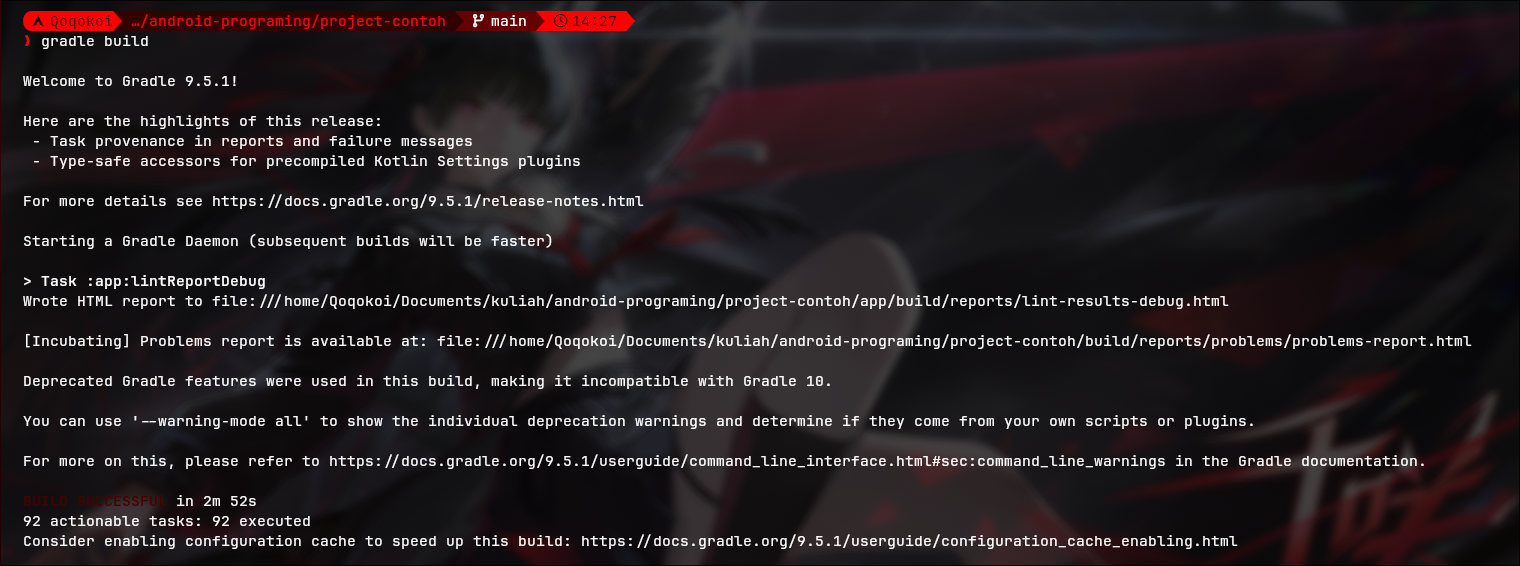
\includegraphics[width=0.9\textwidth]{screenshot_20260614_143036.png}
    \caption{Bukti Log Kompilasi Sukses melalui Gradle CLI}
\end{figure}

\subsection{Deployment ke Perangkat Fisik (ADB Streamed Install)}
Paket biner aplikasi terkompilasi (\texttt{app-debug.apk}) berhasil didistribusikan ke target pengujian melalui interaksi jembatan ADB. Status eksekusi menunjukkan \texttt{Success}, dan aplikasi mampu melakukan \textit{runtime mapping} identitas mahasiswa secara langsung pada perangkat fisik:

\begin{lstlisting}[style=terminal, title={Log ADB Deployment \& Aktivasi Subsistem}]
) adb devices
List of devices attached
452024611067_DafiDevice    device

) adb install app/build/outputs/apk/debug/app-debug.apk
Performing Streamed Install
Success
\end{lstlisting}

\begin{figure}[h!]
  \centering
  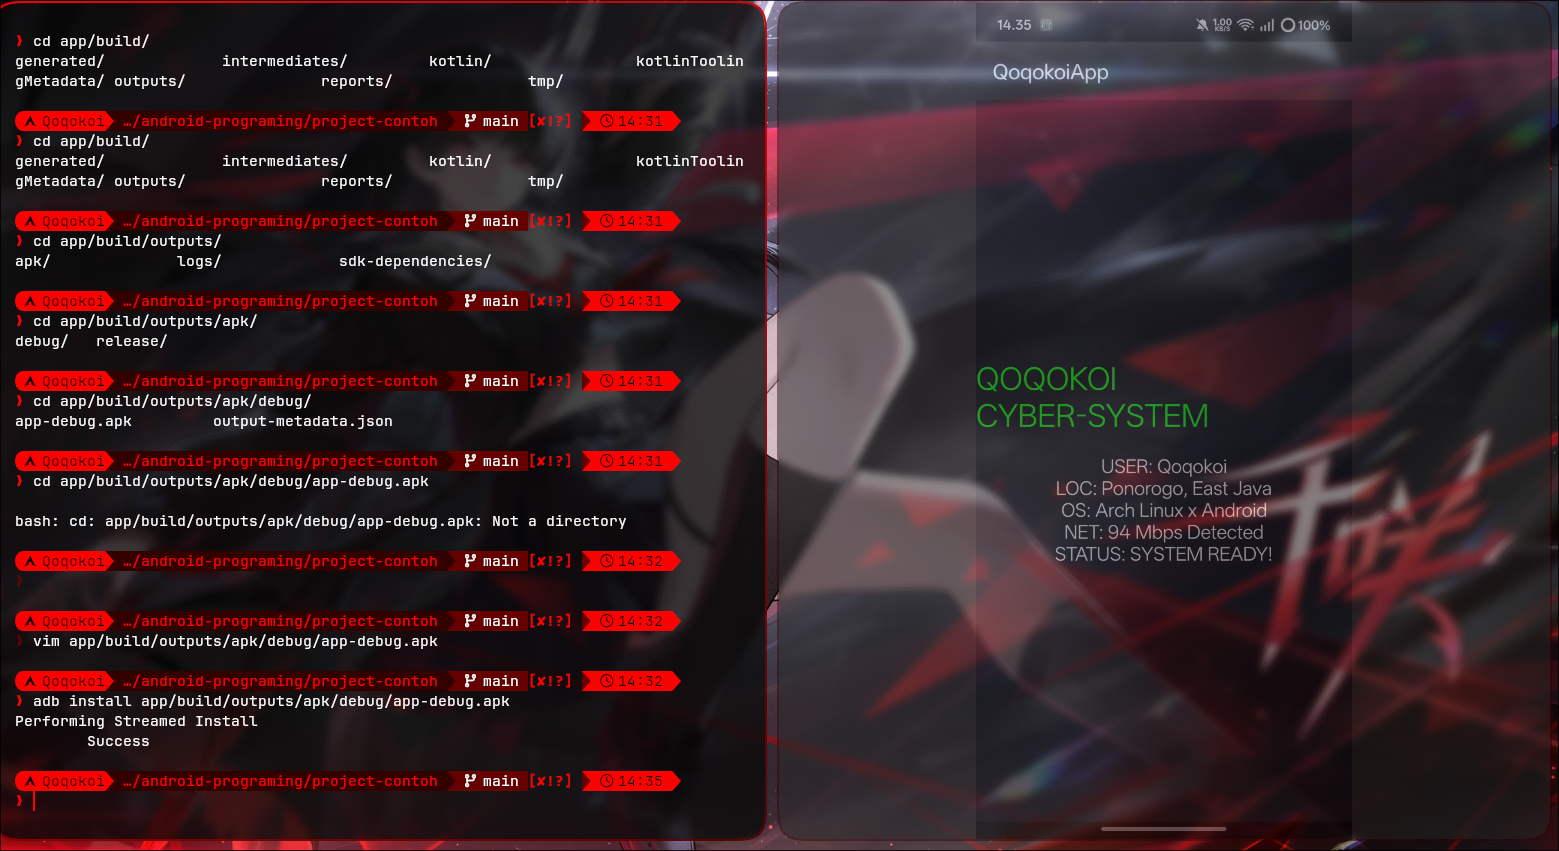
\includegraphics[width=0.9\textwidth]{screenshot_20260614_143540.png}
  \caption{Eksekusi Bersandingan Antara Log ADB Terminal dan Runtime Aplikasi pada Perangkat Target}
\end{figure}

Aplikasi target \textbf{``Qoqokoi App''} berhasil diinisialisasi pada \textit{smartphone} fisik dengan menampilkan status verifikasi lingkungan secara aktual: \texttt{USER: Qoqokoi}, \texttt{OS: Arch Linux x Android}, serta \texttt{STATUS: SYSTEM READY!} yang menandakan subsistem siap dipakai.

% ==================== SECTION 4 ====================
\section{Kesimpulan Kesiapan Sistem}
Melalui seluruh rangkaian pengujian dari hulu ke hilir menggunakan \textit{Pure Terminal Engine} di atas Arch Linux, seluruh komponen utama meliputi Java Development Kit, Android SDK Toolchain, Android Debug Bridge, serta Gradle Compiler Automations dinyatakan telah terkonfigurasi dengan validasi penuh 100\% sukses. Infrastruktur lokal ini siap digunakan untuk menangani seluruh beban kerja praktikum pemrograman aplikasi Android pada masa mendatang tanpa adanya kendala teknis kelayakan sistem.

\end{document}
